\chapter{Contexto y estado del arte}\label{chap:2contexto}

En esta sección se intentarán poner en perspectiva, de una forma no exhaustiva, las distintas razones
históricas que dan lugar a la necesidad de crear un sistema de almacenamiento descentralizado y distribuido como IPFS.
Para ello, se hará un breve repaso histórico de la evolución de Internet y de los protocolos que lo han ido conformando.
Posteriormente, se explicará la tendencia centralista del sistema actual, existente a un nivel intrínseco y estructural,
además de otros problemas que se derivan de esta situación.
Finalmente, se expondrá la propuesta de solución que IPFS ofrece para solventar estos problemas, sobre la que se profundizará en la sección \ref{sect:ipfs}: '\nameref{sect:ipfs}'.

\section{Breve historia de Internet}
\subsection{Predominancia de los protocolos TCP/IP}
La historia de internet está marcada por la competencia entre distintos protocolos de comunicación que buscaban establecerse
como el estándar para intercambiar información entre diferentes redes y sistemas. Uno de los episodios más relevantes de esta
competencia fue la llamada \textit{"Guerra de los protocolos"} \cite{ProtocolWars2023}, en la que el conjunto de protocolos TCP/IP, creado entre los
años 1973 y 1974 por Vint Cerf y Robert Kah, se enfrentó a otras propuestas como OSI, X.25 o SNA\footnote{En la figura \ref{tab:comparacion-protocolos-90} de la página \pageref{tab:comparacion-protocolos-90} se muestra un resumen de las principales características de cada uno de estos protocolos.
}.

TCP/IP logró imponerse a la competencia debido a las siguientes características principalmente:
\begin{itemize}
      \item \textbf{ Interoperabilidad }: La capacidad de TCP/IP para conectarse fácilmente con diferentes tipos de ordenadores y sistemas operativos le otorgaba una ventaja sobre otros protocolos que eran más específicos o limitados en su compatibilidad. Esta característica permitía que diversas tecnologías y plataformas pudieran comunicarse entre sí sin problemas, lo cual era esencial para crear una red global como internet.

      \item \textbf{ Flexibilidad }: TCP/IP podía adaptarse a distintos medios de transmisión, como cables de cobre, fibra óptica o incluso enlaces inalámbricos, lo que facilitaba su implementación en una amplia variedad de entornos y situaciones. Otros protocolos, en cambio, podrían haber requerido modificaciones o adaptaciones específicas para funcionar en diferentes tipos de medios de transmisión.

      \item \textbf{ Resistencia }frente a fallos: TCP/IP fue diseñado para ser robusto en caso de fallos en la red, permitiendo que los paquetes de datos pudieran ser retransmitidos y encontrar rutas alternativas en caso de problemas. Esta capacidad de recuperación era fundamental para garantizar la continuidad y fiabilidad de las comunicaciones en una red global con múltiples nodos y enlaces.

      \item \textbf{ Escalabilidad }: TCP/IP podía soportar el crecimiento de la red al permitir la incorporación de nuevos nodos y enlaces sin afectar negativamente su rendimiento. Su diseño jerárquico y descentralizado facilitaba la expansión de la red y evitaba los cuellos de botella que podrían haberse producido con otros protocolos menos escalables.

\end{itemize}

Estas ventajas hicieron que TCP/IP se convirtiera en la opción preferida frente a otros protocolos, al ser una solución más versátil,
resistente y escalable para la creciente demanda de interconexión entre sistemas y redes en todo el mundo.
Cabe destacar también que era una solución con arquitectura abierta, no propietaria y de uso gratuito, es decir, sin necesidad de pagar licencias por su uso \cite{edwardsFoundationInternetTCP2021}.

Como en toda guerra también hubo un trasfondo político. Este hecho suele ser ignorado al abordarse este tema desde un punto de vista puramente tecnológico.
Y es que en 1980, el Departamento de Defensa de Estados Unidos declaró TCP/IP como el estándar para todas las redes militares \cite{leinerBriefHistoryInternet1999}.
A esto se sumaron numerosas comunidades de investigación y universidades que adoptaron TCP/IP como su protocolo de comunicación, como por ejemplo, Stanford University, donde Vint Cerf colaboró con Robert Kahn en el diseño del protocolo \cite{leinerBriefHistoryInternet1999}; University of California, Los Angeles (UCLA), que participó en el desarrollo temprano y las pruebas de TCP/IP \cite{leinerBriefHistoryInternet1999}; y University College London (UCL), donde el profesor Peter Kirstein promovió el uso de TCP/IP en Europa y su equipo contribuyó al desarrollo y pruebas del protocolo \cite{moriPeterKirsteinObituary2020}.

\begin{figure}[H]
      \centering
      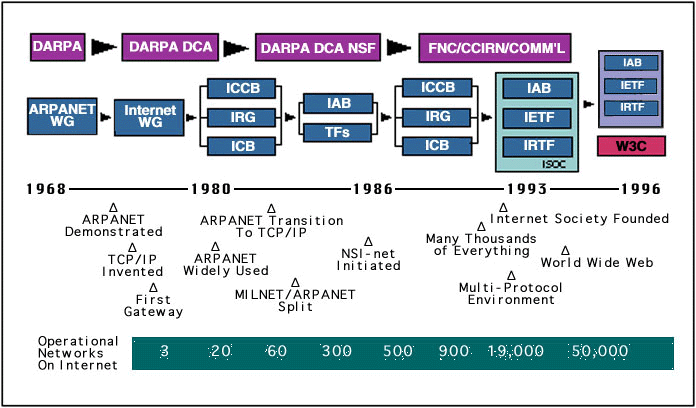
\includegraphics[width=0.8\textwidth]{images/TimelineOfTheInternetProtocols.png}
      \caption[Evolución de los protocolos de Internet]{Evolución de los protocolos de Internet. Fuente \cite{leinerBriefHistoryInternet1999}}
\end{figure}

Esta completa adopción del protocolo se dió por finalizada cuando ARPANET precursor de
internet y financiado por la Agencia de Proyectos de Investigación Avanzados de Defensa
(DARPA), llevó a cabo la transición exitosa de su antiguo protocolo, el Network Control Program
(NCP), a TCP/IP el 1 de enero de 1983 \cite{leinerBriefHistoryInternet1999}.

En resumen, la rápida adopción de la comunidad científica y académica, sumada al respaldo gubernamental consolidaron TCP/IP como el estándar dominante en la industria de las redes de comunicación.

\subsection{La World Wide Web y HTTP}
El modelo TCP/IP asentó una forma de comunicación estándar entre computadores y redes, aunque
este estaba limitado principalmente al mundo académico y científico. No fue hasta la creación de la World Wide Web (WWW)
cuando el Internet concebido como es en la actualidad se convirtió en un fenómeno global y accesible para todo el mundo.

Antes de la WWW, el acceso a la información en Internet se realizaba a través de los protocolos a nivel de aplicación mostrados en la figura \ref{fig:evolucion-protocolos}

\begin{table}[h]
      \small
      \centering
      \begin{tabular}{>{\raggedright}m{3cm}m{10cm}}
            \toprule
            \textbf{Protocolo}                                   & \textbf{Descripción}                                                                                                                                                \\
            \midrule
            FTP (Protocolo de Transferencia de Archivos)         & Utilizado para transferir archivos entre cliente y servidor a través de una red.                                                                                    \\
            \addlinespace
            Telnet                                               & Basado en texto utilizado para el acceso remoto a computadoras y servidores, permitiendo a los usuarios controlarlos a través de una interfaz de línea de comandos. \\
            \addlinespace
            Gopher                                               & Diseñado para buscar y recuperar documentos de manera jerárquica, utilizando una interfaz basada en menús.                                                          \\
            \addlinespace
            SMTP (Protocolo Simple de Transferencia de Correo)   & Utilizado para enviar mensajes de correo electrónico entre servidores y, finalmente, al cliente de correo del destinatario.                                         \\
            \addlinespace
            NNTP (Protocolo de Transferencia de Noticias en Red) & Utilizado para la distribución, consulta y recuperación de artículos de noticias en la red Usenet.                                                                  \\
            \addlinespace
            POP3 (Protocolo de Oficina de Correos 3)             & Utilizado para recuperar mensajes de correo electrónico desde un servidor de correo remoto hasta un cliente de correo local.                                        \\
            \addlinespace
            IMAP (Protocolo de Acceso a Mensajes de Internet)    & Permite a los usuarios acceder y administrar sus mensajes de correo electrónico en un servidor de correo, sin descargarlos a un cliente de correo local.            \\
            \bottomrule
      \end{tabular}
      \caption{Protocolos de capa de aplicación antes de HTTP}
      \label{fig:evolucion-protocolos}
\end{table}

Estos servicios se encuentran en nivel de aplicación dentro del \textit{stack} TCP/IP, como se muestra en la figura \ref{fig:tcpip}.
Algunos de ellos se siguen usando hoy en día, o tienen su caso de uso (IMAP, POP3, FTP), pero en lo referente a archivos,
ofrecían métodos básicos de navegación y compartición. Carecían de la capacidad de inter-conectar documentos de manera intuitiva y visual.
\footnote{Cabe destacar que en esta época, los documentos eran principalmente texto plano, sin formato, y no existía la posibilidad de incluir imágenes o vídeos.}

\usetikzlibrary{shapes,arrows,positioning, babel}
\begin{figure}[h!]
      \centering
      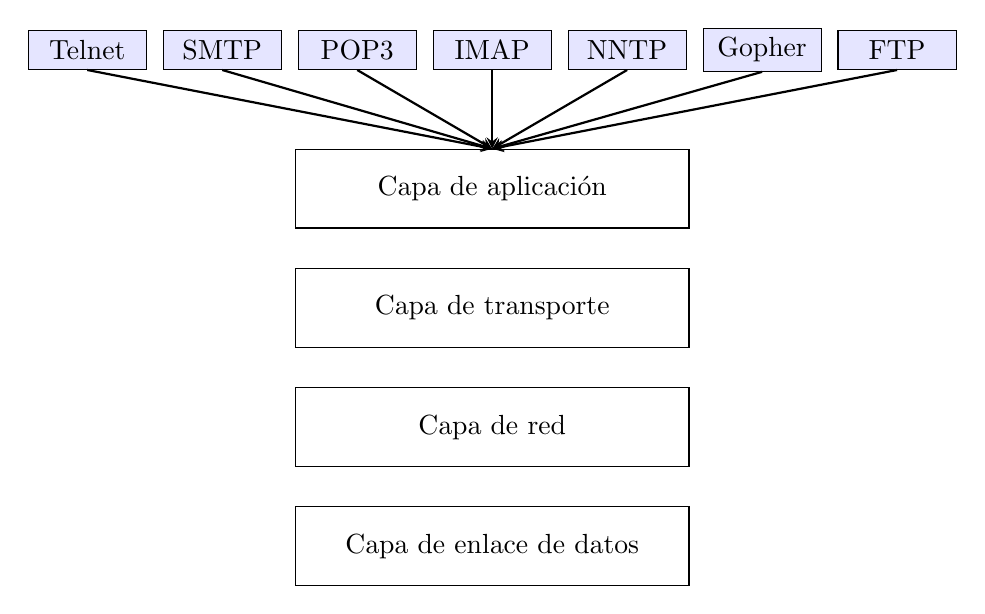
\begin{tikzpicture}
            % Estilos
            \tikzstyle{layer}=[draw, rectangle, minimum height=1cm, minimum width=5cm, text centered]
            \tikzstyle{app_protocol}=[draw, rectangle, minimum height=0.5cm, minimum width=1.5cm, text centered, fill=blue!10]
            \tikzstyle{arrow}=[->,>=stealth, thick]

            % Nodos
            \node[layer] (application) {Capa de aplicación};
            \node[layer, below=0.5cm of application] (transport) {Capa de transporte};
            \node[layer, below=0.5cm of transport] (network) {Capa de red};
            \node[layer, below=0.5cm of network] (link) {Capa de enlace de datos};

            \node[app_protocol, above=1cm of application.north] (imap) {IMAP};
            \node[app_protocol, left=0.2cm of imap] (pop3) {POP3};
            \node[app_protocol, right=0.2cm of imap] (nntp) {NNTP};
            \node[app_protocol, left=0.2cm of pop3] (smtp) {SMTP};
            \node[app_protocol, right=0.2cm of nntp] (gopher) {Gopher};
            \node[app_protocol, left=0.2cm of smtp] (telnet) {Telnet};
            \node[app_protocol, right=0.2cm of gopher] (ftp) {FTP};

            % Flechas
            \draw[arrow] (imap.south) -- (application.north);
            \draw[arrow] (pop3.south) -- (application.north);
            \draw[arrow] (nntp.south) -- (application.north);
            \draw[arrow] (smtp.south) -- (application.north);
            \draw[arrow] (gopher.south) -- (application.north);
            \draw[arrow] (telnet.south) -- (application.north);
            \draw[arrow] (ftp.south) -- (application.north);
      \end{tikzpicture}
      \caption{Capas del protocolo TCP/IP mostrando algunos protocolos de la capa de aplicación}
      \label{fig:tcpip}
\end{figure}

En 1989, el científico británico Tim Berners-Lee propuso la creación de la WWW, un sistema de información
global que permitiría a los usuarios navegar y acceder a documentos interconectados mediante
enlaces. Estos documentos, conocidos como páginas web, se almacenarían en computadoras conectadas a la red y podrían ser accedidos
a través de un programa especial llamado navegador web, que interpretaría el código de las páginas y mostraría su contenido al usuario.
\\HTML (Hyper Text Markup Language) es el lenguaje que describe estos documentos. Permite enlazar documentos entre sí mediante hipervínculos. Un hipervínculo es una referencia unidireccional en un documento electrónico que entrelaza diferentes documentos o secciones entre sí. Los usuarios tienen la oportunidad de seguir estos enlaces con tan solo un clic en el texto ancla (texto enlazado) para navegar a los documentos o las secciones correspondientes\cite{Hiperenlace2023}.
Aunque es un concepto simple y con el que cualquier persona en la actualidad esta familiarizada este factor dictamina la forma
en la que se usa internet en la actualidad. Los usuarios de internet interactúan con el contenido en internet mediante estos enlaces.
\\La WWW se basó en tres tecnologías clave: HTML, un lenguaje de marcado para crear páginas web; HTTP, un protocolo para solicitar y transferir recursos a través de la web; y URL, un sistema de direcciones para localizar recursos en la web\cite{leinerBriefHistoryInternet1999}. Y es este último el que genera una gran problemática que resuelve IPFS.

URL significa Uniform Resource Locator, que se traduce al español como Localizador Uniforme de Recursos. Es un sistema de direcciones utilizado en la web para localizar de manera única recursos como páginas web, imágenes, videos y otros archivos. Una URL consta de varios componentes, incluyendo el esquema (como "http://" o "https://"), el nombre de dominio (como "www.ejemplo.com"), la ruta del recurso y otros parámetros opcionales.

\setlength{\parskip}{10pt}
Sin embargo, a medida que la web ha crecido en tamaño y complejidad, el enfoque de direccionamiento basado en la ubicación física
de los servidores puede presentar limitaciones. Por ejemplo, si un recurso se encuentra en una URL específica y esa URL cambia o
el servidor deja de estar disponible, el acceso al recurso se verá comprometido.

IPFS aborda este problema mediante el uso de un sistema de direccionamiento basado en el contenido, en lugar de la ubicación. En
IPFS, cada archivo y bloque de datos se identifican mediante su contenido, utilizando una función hash criptográfica. Esto
permite que los archivos y bloques se puedan encontrar y acceder de forma fiable, independientemente de su ubicación física.

Esto permite a IPFS ofrecer una serie de ventajas sobre el sistema de direccionamiento basado en la ubicación de la web
tradicional, como la resistencia a la censura, la persistencia de los datos y la verificabilidad del contenido.
En la siguiente sección se profundizará en estas ventajas y en cómo IPFS las hace posibles.

\section{IPFS como alternativa a HTTP}\label{sect:ipfs}

\subsection{Introducción}
% Briefly introduce the concept of IPFS and its significance in the modern era of the internet.
% Provide a background on why IPFS was created and its aims.
IPFS fue presentado al mundo en 2014 por Juan Benet, en un informe técnico titulado
\textit{IPFS - Content Addressed, Versioned, P2P File System}\cite{benetIPFSContentAddressed2014}.
Benet presenta el concepto de IPFS y su proposición de crear un sistema de archivos
distribuido y descentralizado que permita a los usuarios almacenar y compartir archivos de forma segura y confiable.

Benet es también el fundador de Protocol Labs\cite{ProtocolLabs}, una empresa dedicada a la creación de protocolos de código abierto para la Web3.
IPFS es un proyecto de código abierto y pese a que Protocol Labs está detrás de este, no es el único contribuidor a su desarrollo. Esto es otro
de los puntos fuertes de IPFS, la comunidad que lo rodea. En la sección \ref{sect:ecosistema}: '\nameref{sect:ecosistema}' se profundiza en este aspecto.

En IPFS, cada archivo se identifica de manera única a través de su contenido mediante un hash criptográfico. Esto significa que
cualquier nodo en la red puede actuar como un proveedor de contenido al almacenar y compartir archivos, permitiendo una mayor
disponibilidad y un internet verdaderamente descentralizado. En lugar de depender de un único servidor web para acceder a un
recurso, los usuarios pueden obtener el contenido de cualquier nodo que tenga ese recurso en particular.

Estos identificadores de contenido se conocen como CID (Content Identifier). Dado que un CID es un puntero que señala a un contenido particular, se puede usar un CID en vez de URL en un enlace. De esta manera
se puede acceder a un recurso de manera fiable, independientemente de su ubicación física, mientras haya algún otro nodo de la red que el contenido que buscamos.

\subsection{Fundamentos}\label{sect:fundamentos}
% Describe the key concepts and terminologies involved in IPFS, such as Content-addressed, Peer-to-peer (P2P) network, and Merkle DAG.
% Explain how these concepts work together to make IPFS a decentralized and distributed file system.
IPFS opera a través de tres principios fundamentales que marcan una diferencia significativa con respecto a los sistemas de archivos convencionales: direccionamiento por contenido, red peer-to-peer y el grafo acíclico dirigido de Merkle (Merkle DAG).


\textbf{Direccionamiento por Contenido:} En IPFS, los archivos no se ubican por su dirección sino por su contenido. Cada archivo posee un
identificador único, denominado CID (Content Identifier), generado a partir de un hash criptográfico de su contenido. Esta característica
asegura la inmutabilidad de los archivos, es decir, los archivos no pueden ser alterados sin modificar su CID. Adicionalmente, el
direccionamiento por contenido favorece la deduplicación, dado que archivos con contenido idéntico compartirán el mismo CID, lo que conlleva a
su almacenamiento único dentro de la red.

\begin{figure}[H]
      \begin{minted}[fontsize=\small]{bash}
$ ipfs add somefile # ejemplo de comando para añadir un archivo a IPFS mediante la CLI de IPFS
added QmVtuHo6C7NUonYTYUNbmgGxvSwrTVGXuahJxhxnoSxPpM somefile
\end{minted}
      \caption{Ejemplo de CID generado por IPFS}
      \label{fig:ipfs-add}
\end{figure}

\textbf{Red Peer-to-Peer:} IPFS se basa en una red descentralizada en la que cada integrante, o nodo, puede interactuar directamente con cualquier otro nodo, sin la necesidad de intermediarios o servidores centrales. Los nodos funcionan tanto como proveedores como consumidores de contenido, guardando y compartiendo fragmentos de archivos con otros nodos. Esta red peer-to-peer hace que el contenido sea más accesible y resistente a la censura, al evitar la existencia de un único punto de fallo o control.
\begin{figure}[H]
      \centering
      
\includegraphics[width=\linewidth]{images/centralvsdecentral.png}
      \caption{Red centralizada en comparación con una red descentralizada}
      \label{fig:centralvsdecentral}
\end{figure}

\textbf{Grafo Acíclico Dirigido de Merkle (Merkle DAG):} Los archivos y sus relaciones dentro de IPFS se representan mediante una estructura de datos conocida como Merkle DAG. Un Merkle DAG es un grafo donde cada nodo tiene un identificador único (CID) que se genera a partir de su contenido y el de sus nodos hijos. Los nodos pueden ser hojas o nodos intermedios, dependiendo de si tienen o no nodos hijos. Los nodos hoja contienen datos binarios de los archivos, mientras que los nodos intermedios contienen enlaces a otros nodos. Los nodos intermedios permiten dividir archivos grandes en bloques más pequeños y formar estructuras jerárquicas, como directorios o sistemas de archivos. El Merkle DAG facilita la verificación de integridad y autenticidad de los archivos, dado que cualquier cambio en el contenido o en los enlaces se refleja en el CID del nodo afectado y sus ancestros.

Cada uno de estos conceptos se profundizará dentro del apartado correspondiente a continuación.

\subsection{Arquitectura}
% Describe the core components of IPFS architecture, such as IPFS node, IPFS client, IPFS gateway, and IPFS cluster.
% Explain the role of each component in the IPFS network.
IPFS es un conjunto de protocolos de código abierto que combina múltiples conceptos existentes de redes
peer-to-peer (P2P), datos enlazados y otras áreas para permitir que los participantes intercambien fragmentos de
archivos.

Estos conceptos concretados en protocolos forman distintos niveles de abstracción, cada uno de los cuales se puede utilizar de forma independiente y conforman la arquitectura de IPFS, también conocido como el \textit{stack} de protocolos de IPFS.
Esta pila de protocolos tiene cierto parecido al modelo OSI (Open Systems Interconnection), que es un modelo conceptual que caracteriza y
estandariza las funciones de comunicación de un sistema de comunicación o red de computadoras, dividiéndolo en siete capas. Cada capa se encarga
de un aspecto específico de la comunicación. La figura \ref{fig:osi} muestra el modelo OSI y las funciones de cada capa.

\begin{figure}[H]
      \centering
      \vspace{5pt} % Reduce 1cm de espacio antes de la figura
      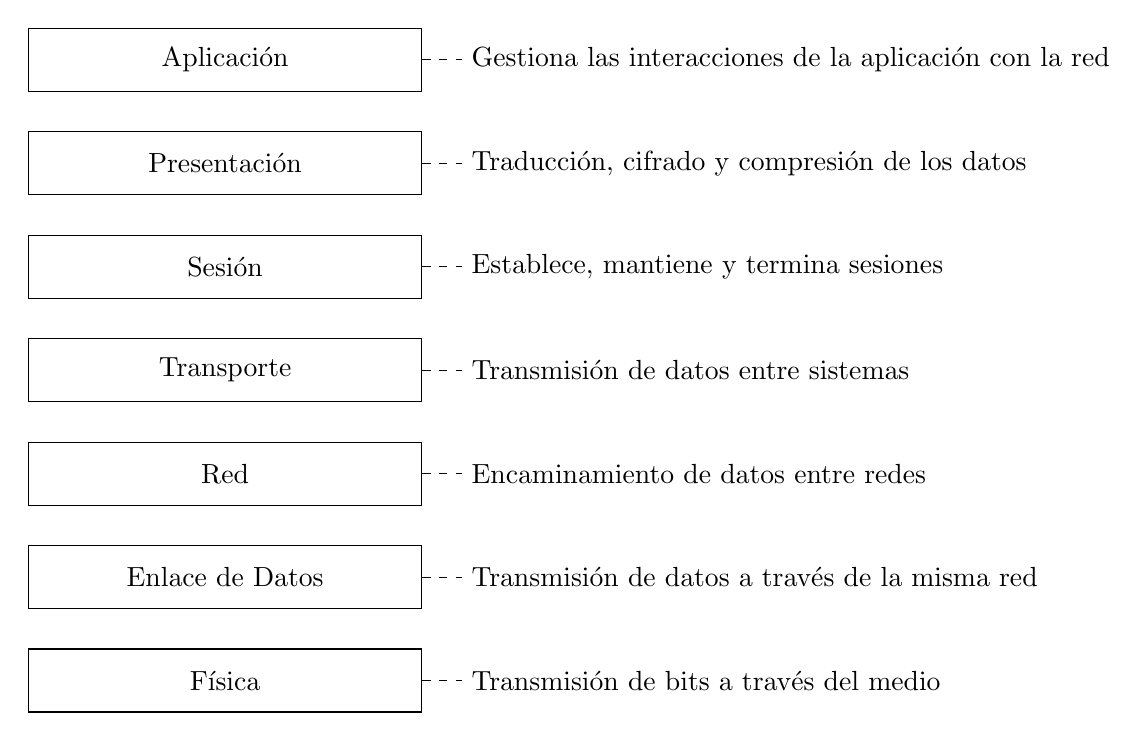
\begin{tikzpicture}[
                  every node/.style={rectangle,draw,minimum width=5cm, minimum height=0.8cm,align=center},
                  node distance=0.5cm and 0.5cm,
                  desc/.style={xshift=0cm, align=center, draw=none},
            ]
            \node (a1) {Aplicación};
            \node[desc] (d1) [right=of a1] {Gestiona las interacciones de la aplicación con la red};
            \draw[dashed] (a1.east) -- (d1.west);

            \node (a2) [below=of a1] {Presentación};
            \node[desc] (d2) [right=of a2] {Traducción, cifrado y compresión de los datos};
            \draw[dashed] (a2.east) -- (d2.west);

            \node (a3) [below=of a2] {Sesión};
            \node[desc] (d3) [right=of a3] {Establece, mantiene y termina sesiones};
            \draw[dashed] (a3.east) -- (d3.west);

            \node (a4) [below=of a3] {Transporte};
            \node[desc] (d4) [right=of a4] {Transmisión de datos entre sistemas};
            \draw[dashed] (a4.east) -- (d4.west);

            \node (a5) [below=of a4] {Red};
            \node[desc] (d5) [right=of a5] {Encaminamiento de datos entre redes};
            \draw[dashed] (a5.east) -- (d5.west);

            \node (a6) [below=of a5] {Enlace de Datos};
            \node[desc] (d6) [right=of a6] {Transmisión de datos a través de la misma red};
            \draw[dashed] (a6.east) -- (d6.west);

            \node (a7) [below=of a6] {Física};
            \node[desc] (d7) [right=of a7] {Transmisión de bits a través del medio};
            \draw[dashed] (a7.east) -- (d7.west);
      \end{tikzpicture}
      \caption{Modelo OSI}
      \label{fig:osi}
\end{figure}

El stack de IPFS aunque parecido no es exactamente igual, pero el modelo OSI es una buena referencia para entender el de IPFS.
En la figura \ref{fig:ipfs} se muestra el stack de protocolos de IPFS.

\begin{figure}[H]
      \centering
      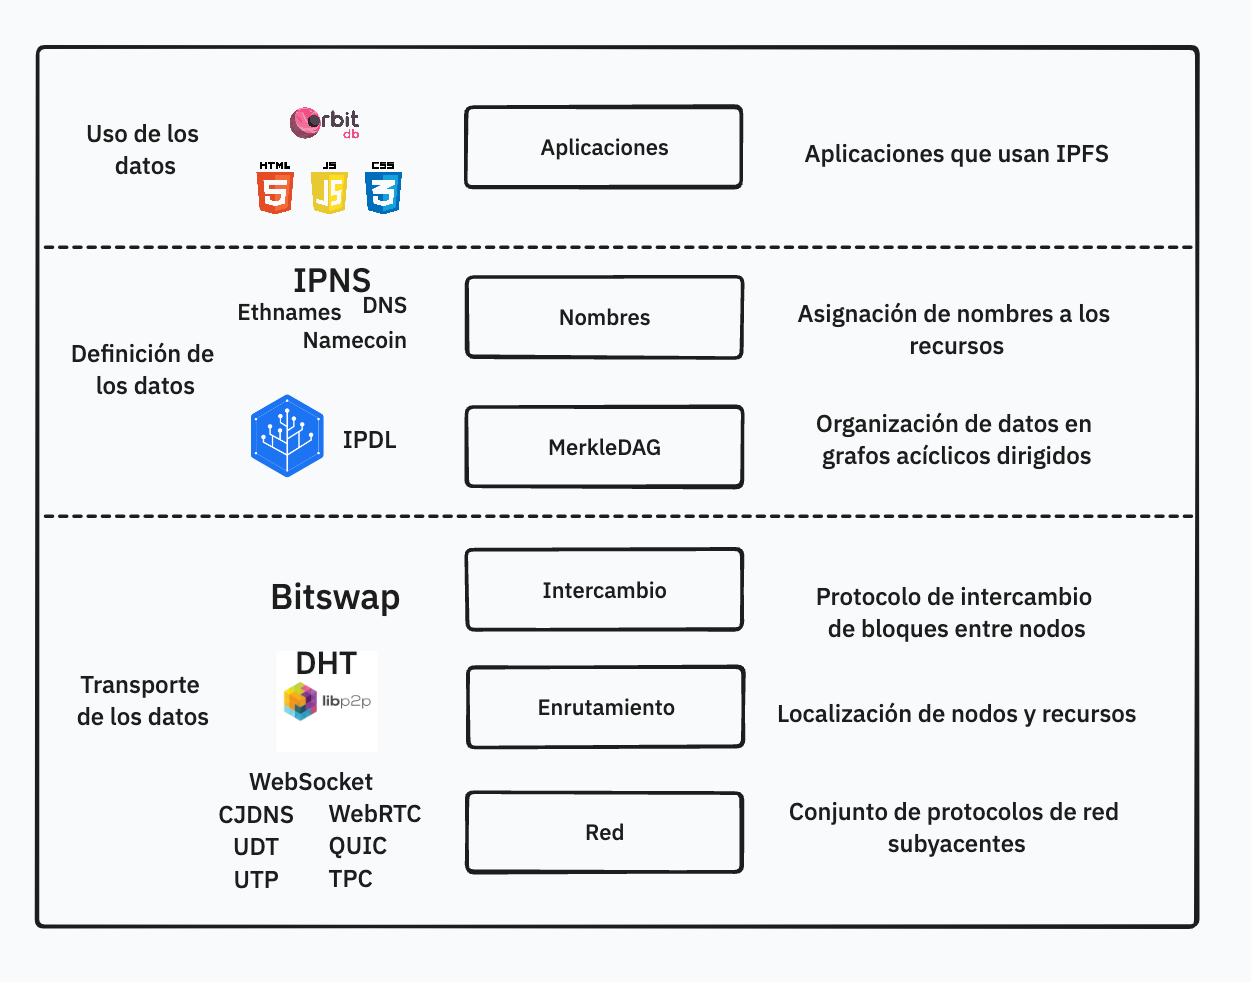
\includegraphics[width=\linewidth]{images/ipfs-stack.png}
      \caption{Stack de protocolos IPFS}
      \label{fig:ipfs}
\end{figure}

Como se puede observar, este stack podría subdividirse en tres grupos según la funcionalidad que brinda cada capa.
Este diseño en capas subdivido en componentes independientes permite que estos pueden ser ampliados o reemplazados
cuando sea necesario. Esta modularidad en el diseño está respaldada por una biblioteca de redes P2P llamada libp2p\cite{WhatLibp2p}.
\\libp2p es una biblioteca modular de redes P2P para la dirección de procesos, con un
enfoque en los procesos de transferencia de datos, con soporte para implementaciones de varios protocolos de red y de capa de
transporte. libp2p también integra protocolos para la ruta de contenido y pares a través de una Tabla Hash Distribuida (DHT),
un protocolo de publicación-suscripción y un protocolo de intercambio de contenido llamado Bitswap.\cite{doanDecentralisedCloudStorage2022}.

\subsubsection{Capa de red}
En la capa de red encontramos los protocolos de transporte de red mediante los cuales los nodos en la red se pueden comunicar. Estos protocolos provienen de libp2p\cite{labsLibp2pConnectivity} y son los siguientes:
\begin{itemize}
      \item \textbf{TCP}: proporciona una entrega de datos confiable, ordenada y con control de errores sobre redes IP.
      \item \textbf{UDP}: proporciona una entrega de datos simple, sin conexión y no confiable sobre redes IP.
      \item \textbf{QUIC}: Un protocolo de transporte multiplexado y seguro que se ejecuta sobre UDP, proporcionando flujos confiables, de baja latencia y cifrados.
      \item \textbf{WebSockets}: Un protocolo que permite la comunicación bidireccional entre un navegador web y un servidor sobre TCP.
      \item \textbf{WebRTC}: Un protocolo que permite la comunicación en tiempo real entre navegadores web mediante conexiones peer-to-peer.
\end{itemize}

Debido a esta gran variedad de protocolos de transporte, libp2p proporciona una forma de identificar el transporte que se esté usando mediante
direcciones \textit{multiaddr}.
Los multiaddresses son una forma de representar las direcciones de red como encapsulaciones de protocolos arbitrarios. Estos multiaddresses admiten direccionar
para cualquier protocolo de red. Siguen una sintaxis simple, lo que los hace fáciles de analizar y construir.

En IPFS, se utilizan los multiaddresses para identificar y localizar los nodos en la red. Cada nodo tiene un identificador único llamado peerID, que es el hash de su clave pública. Además, los nodos tienen una o más direcciones de red que combinan protocolos y valores para indicar cómo conectarse a ellos. Por ejemplo, una dirección de red podría ser /ip4/1.2.3.4/tcp/4001/ipfs/QmFoo, lo que significa que el nodo QmFoo está escuchando conexiones TCP en el puerto 4001 utilizando la dirección IP 1.2.3.4.

Los multiaddresses se pueden encapsular entre sí para crear capas de transporte más complejas. Por ejemplo, se puede utilizar /dns4/example.com/tcp/1234/tls/ws/tls para indicar una conexión segura con WebSockets sobre TLS utilizando el dominio example.com y el puerto 1234.

La amplia variedad de protocolos de transporte disponibles garantiza la adaptabilidad de IPFS, ya que los nodos pueden utilizar múltiples protocolos de transporte simultáneamente y cambiar entre ellos según las condiciones de la red. Esto significa que las opciones de transporte de un nodo dependen del entorno en el que se ejecute. Por ejemplo, en un navegador web, solo se pueden utilizar WebSockets y WebRTC, mientras que en otros entornos se pueden utilizar todos los protocolos mencionados anteriormente, siempre que sean compatibles.

El peerID

\subsubsection{Enrutamiento y descubrimiento de nodos}
\textbf{Descubrimiento de nodos:}
\\El descubrimiento de pares es el proceso de encontrar y anunciar servicios a otros nodos disponibles en una red P2P. Se puede realizar utilizando diversos protocolos, por ejemplo la difusión de mensajes a todos los nodos de la red o
utilizar un nodo de arranque para proporcionar una lista de pares conocidos.

\textbf{Enrutamiento}:
\\Por otro lado, enrutamiento se refiere a encontrar la ubicación específica de otro nodo de la red. Esto se realiza
típicamente mediante el mantenimiento de una tabla de enrutamiento u otra estructura de datos similar que realiza un
seguimiento de la topología de la red. En el caso de IPFS se usa una tabla de hash distribuida conocida como DHT (Distributed
hash table).

En una red P2P, se utilizan diversos algoritmos para encontrar los pares cercanos a un ID de par específico. Un nodo puede
emplear un algoritmo de enrutamiento para localizar a otro nodo en particular y utilizar esa nodo para descubrir otro nodos
que este conozca.

En la práctica, la distinción entre el enrutamiento y el descubrimiento de nodos no siempre está clara, de hecho suelen ocurrir simultáneamente.

Los protocolos principales que usa IPFS y libp2p son:

\begin{itemize}
      \item \textbf{ping}: Protocolo de comprobación de disponibilidad. Los nodos pueden utilizarlo para verificar la conectividad y el rendimiento entre ellos.
      \item \textbf{autonat}: Protocolo de detección de NAT. Asiste a los nodos en la identificación de su accesibilidad desde internet, esto es útil para detectar si los nodos que se encuentran ocultos detrás de un NAT o de un firewall \cite{AutoNAT}.
      \item \textbf{identify}: Protocolo para el intercambio de claves y direcciones con otros nodos. Facilita el intercambio de información esencial, como los protocolos soportados, las claves públicas, las direcciones, etc.
      \item \textbf{kademlia}: Implementa una tabla hash distribuida para el almacenamiento descentralizado y la recuperación de información de nodos y contenidos.
      \item \textbf{mdns}: Protocolo de descubrimiento de nodos locales con cero configuración, usando DNS de multidifusión. Ofrece un mecanismo para que los nodos en la misma red local se descubran entre sí sin configuración previa.
      \item \textbf{Circuit Relays}: Es un protocolo que facilita a los nodos el reenvío de tráfico en nombre de otros nodos que no tienen un acceso directo entre ellos\cite{CircuitRelay}.
      \item \textbf{rendezvous}: Un protocolo de encuentro que se utiliza como un punto común entre dos rutas.
            Los puntos de encuentro son típicamente nodos que están bien conectados y son estables en una red, y pueden manejar grandes cantidades de tráfico y datos. Sirven como un centro para que los nodos se descubran. De los pocos mecanismos centralizados que usa libp2p \cite{Rendezvous}.
      \item \textbf{pubsub}: Es una interfaz PubSub para libp2p, diseñada para establecer una base para la comunicación de mensajes mediante un patrón de publicación y suscripción entre los nodos de la red libp2p. Existen diferentes implementaciones de este protocolo, como FloodSub, GossipSub que proporcionan
            diferentes ventajas.
\end{itemize}

Como se ha comentado, libp2p ofrece varias formas de enrutamiento y descubrimiento de nodos, IPFS utiliza todos ellos en sus distintas
configuraciones en aras de intentar establecer conexiones con otros nodos de la red, y es por esto que depende del contexto la combinación
de ellos que se use.

\subsubsection{Mecanismo de intercambio de contenido}

\textbf{Bitswap:} Es un protocolo de intercambio de contenido que se ejecuta sobre una red P2P. Bitswap permite a los nodos intercambiar bloques de datos entre
sí. Los nodos pueden solicitar bloques de datos a otros nodos y compartir los bloques que ya tienen. Bitswap utiliza un mecanismo de intercambio de deuda para
garantizar que los nodos intercambien bloques de datos de manera justa y equitativa. Los nodos pueden intercambiar bloques de datos de manera eficiente, ya que
Bitswap mantiene un registro de los bloques que cada nodo tiene y los bloques que necesita.

Bitswap es el algoritmo de intercambio de bloques, pero para realizar este intercambio primero se debe saber qué nodos pueden proveer los bloque que se buscan.
Esto es posible gracias a la DHT. En IPFS la DHT se utiliza principalmente con dos funciones:
% enumerated list with numbers
\begin{enumerate}
      \item \textbf{Enrutamiento:} se ha explicado en la subsección anterior.
      \item \textbf{Anuncios de provisión/consumición de contenido:} Los nodos publican en la DHT los bloques de datos que tienen disponibles. Esto permite a otros nodos saber quién tiene los bloques de datos que están buscando. Esta tabla de hash se distribuye por la red mediante Kademlia.
\end{enumerate}

Sobre el segundo, que es el concierne dentro del mecanismo de intercambio de contenido: Cada nodo tiene dos lista de bloques (CIDs). Bloques que posee y puede
proporcionar, y bloques que desea obtener.
\begin{itemize}
      \item Al recibir una lista de deseos, una entidad que use Bitswap debería procesarla eventualmente y responder al solicitante con información sobre el bloque o el bloque en sí.
      \item Al recibir bloques, el nodo consumidor debe enviar una notificación de cancelación al resto de nodos a los que ha pedido estos bloques, señalando que  ya no los desea.
\end{itemize}

Dentro de la configuración de un nodo IPFS podemos encontrar los protocolos soportados
\begin{minted}[fontsize=\small]{json}
"ID": "12D3KooWDM93Kdoiv7vRRoRCi8fYnPwvWtTi39MjXF8rbEt7S4iJ",
"PublicKey": "CAESIDR1ONYFE5I7Qo+9+rr6o+yPk88GE5cR63dJ9RVn++Ev",
"Addresses": [
"/ip4/127.0.0.1/tcp/4001/p2p/12D3KooWDM93Kdoiv7vRRoRCi8fYnPwvWtTi39MjXF8rbEt7S4iJ",
"/ip4/127.0.0.1/udp/4001/quic-v1/p2p/12D3KooWDM93Kdoiv7vRRoRCi8fYnPwvWtTi39MjXF8rbEt7S4iJ",
"/ip4/127.0.0.1/udp/4001/quic/p2p/12D3KooWDM93Kdoiv7vRRoRCi8fYnPwvWtTi39MjXF8rbEt7S4iJ",
"/ip4/192.168.119.108/udp/4001/quic-v1/p2p/12D3KooWDM93Kdoiv7vRRoRCi8fYnPwvWtTi39MjXF8rbEt7S4iJ",
"/ip6/::1/udp/4001/quic-v1/webtransport/certhash/uEiDBbRfNYfXkxh-dTMk7-90pZjn9Ix8nD8Qb2Xsa2y0GXw/certhash/uEiAQHfIKUBbqVLM-ztuxLqV9brJ-qcZ5SOmDNcra-KyMoQ/p2p/12D3KooWDM93Kdoiv7vRRoRCi8fYnPwvWtTi39MjXF8rbEt7S4iJ",
"/ip6/::1/udp/4001/quic/p2p/12D3KooWDM93Kdoiv7vRRoRCi8fYnPwvWtTi39MjXF8rbEt7S4iJ"
],
"AgentVersion": "kubo/0.20.0/b8c472500",
"ProtocolVersion": "ipfs/0.1.0",
"Protocols": [
"/floodsub/1.0.0",
"/ipfs/bitswap",
"/ipfs/bitswap/1.0.0",
"/ipfs/bitswap/1.1.0",
"/ipfs/bitswap/1.2.0",
"/ipfs/id/1.0.0",
"/ipfs/id/push/1.0.0",
"/ipfs/lan/kad/1.0.0",
"/ipfs/ping/1.0.0",
"/libp2p/circuit/relay/0.2.0/stop",
"/libp2p/dcutr",
"/libp2p/fetch/0.0.1",
"/meshsub/1.0.0",
"/meshsub/1.1.0",
"/x/"
]
\end{minted}

\subsection{Modelo de datos}
% Explain the IPFS data model, which involves content addressing and hash-based naming.
% Discuss the benefits of the IPFS data model, such as data integrity, data verifiability, and content-based addressing.
\subsection{Distribución de contenido}
% Describe how IPFS handles content distribution and how it differs from the traditional client-server model.
% Explain how IPFS content distribution works in a P2P network.

\section{Ecosistema en torno a IPFS}\label{sect:ecosistema}

\subsection{Introducción}
% Introduce the concept of the IPFS ecosystem and why it is important.
% Briefly discuss the role of the ecosystem in the development and adoption of IPFS.
\subsection{Proyectos basados en IPFS} % Hablar de las DAPPS
% Provide an overview of the various IPFS projects that exist.
% Categorize the projects into different areas of application, such as storage, web hosting, content distribution, and decentralized applications (dApps).
% Provide examples of notable projects in each category and briefly describe their goals and features.
\subsection{Herramientas y librerías de IPFS}
% Discuss the various tools and libraries that are available to developers working with IPFS.
% Categorize the tools and libraries into different areas, such as API clients, command-line interfaces, development frameworks, and libraries for integrating IPFS into other applications.
% Provide examples of notable tools and libraries in each category and briefly describe their features and capabilities.
\subsection{Comunidades en torno a IPFS}
% Discuss the various communities that exist around IPFS.
% Categorize the communities into different areas, such as developer communities, user communities, and governance communities.
% Provide examples of notable communities in each category and briefly describe their goals and activities.
\subsection{Integraciones de IPFS}
% Discuss the various ways in which IPFS is being integrated with other technologies and platforms.
% Provide examples of notable integrations, such as with Ethereum, Filecoin, and the InterPlanetary Naming System (IPNS).
% Discuss the potential benefits of these integrations and their implications for the broader ecosystem.
